\chapter{Técnicas de desagrupamento} \label{Cap_4}



Uma amostragem dita representativa é aquela que guarda as mesmas proporções e informações da população. No caso de amostragens espaciais nem sempre podemos resguardar posições espaciais equivalentes entre as amostras. Na mineração temos problemas relacionados com a topografia, áreas de proteção ambiental entre outros motivos que tornam a amostragem impossível em certas áreas. Além disso, por motivos econômicos, é de interesse amostrar áreas que são mais econômicas do que áreas pobres do depósito mineral. Para garantir estatísticas não enviesadas do objeto de estudo utilizamos técnicas de desagrupamento que permitem dar pesos diferenciados para cada amostra durante o cálculo das estatísticas. Note que as técnicas de desagrupamento não devem nunca alterar o valor da amostra considerada, mas apenas a estatística, como por exemplo o valor médio, a variância, a frequência do histograma, etc.

\section{Estatísticas desagrupadas} \label{demons_krig} 

Uma estatística desagrupada é aquela em que os valores das amostras recebem um determinado peso associado. A mais comum delas é a média declusterizada, demonstrado na equação \eqref{estatitc_declus}

\begin{equation}\label{estatitc_declus}
	\overline{Z_{d}} = \sum_{i=1}^{n} \rho _{i}z_{i}
\end{equation}

Em que $\rho _{i}$ é o peso associado a cada valor de amostra $z_{i}$. Cada um dos pesos do valor médio de Z são definidos por alguma técnica de desagrupamento como será visto em seções posteriores. Da mesma forma a variância desagrupada pode ser determinada por \eqref{var_declus}
 
 \begin{equation}\label{var_declus}
 Var_{d}(Z) = \sum_{i=1}^{n} \rho _{i} \left( z_{i} - \overline{Z_{d}} \right)^2
 \end{equation}
 
 Uma estatística não enviesada é aquela que seu valor esperado tende a convergir para o valor do parâmetro a ser estimado. No caso das estatísticas declusterizadas temos a condição de que a soma dos ponderadores deve ser igual a 1. Isso pode ser provado om a seguinte demonstração
 
 \begin{proof}
 	$E(\overline{Z_{d}}) = E\left(  \sum_{i=1}^{n} \rho _{i} Z_{i} \right)= m$\\
 	$E(\overline{Z_{d}}) =  \sum_{i=1}^{n} E(\rho _{i} Z_{i}) = m $\\
 	$E(\overline{Z_{d}}) =  \sum_{i=1}^{n} \rho _{i}E( Z_{i}) = m $\\
 	$E(\overline{Z_{d}}) =  \sum_{i=1}^{n} \rho _{i}m = m $\\
 	$ \sum_{i=1}^{n} \rho _{i} = 1 $
 	
 \end{proof}
 
 Essa mesma demonstração ocorre também quando definimos condições para os pesos de krigagem. 
 
 O histograma ponderado também é uma ferramenta importante para a análise estatística de dados desagrupados. Neste caso cada frequência de cada classe é alterada segundo a equação \eqref{pesos_histogram}
 
  \begin{equation}\label{pesos_histogram}
  freq = \frac{\sum_{j=1}^{p} \rho _{i}  z_{j}}{\sum_{i=1}^{n} \rho _{i}  z_{i}} 
  \end{equation}
  
  Em que p é o número de elementos contidos dentro da classe e $z_{j}$ são os valores contidos em cada classe. O valor n é relativo ao número de todas as amostras consideradas e $z_{i}$ é o valor de cada amostra.
 
 \section{Definindo os pesos de desagrupamento}
 
 \subsection{Método dos polígonos de influência}
 
 O primeiro método para encontrar pesos para cada uma das amostras é conhecido como polígonos de influência ou de Thyssen. O objetivo é encontrar uma área convexa para cada uma das amostras contendo a região de influência. Para o caso tridimensional os polígonos se transformam em um poliedro de influência, sendo muito mais complexo a determinação matemática do volume de influência, tornando da metodologia muito mais relevante e desejável para casos bidimensionais. Computacionalmente os polígonos ou poliedros de influência podem ser determinados dividindo o espaço entre as amostras por células, sendo a definição da área ou do volume condicionada ao tamanho da célula, ou seja, quanto menor for a dimensão, maior será a resolução das regiões de influência.
 
 A figura \eqref{tyssen1} demonstra o primeiro passo para se determinar o polígono de Thyssen manualmente. Divide-se as amostras em dois subespaços determinados pela equidistância entre as amostras.
 
\begin{figure}[H]
 	\centering
 	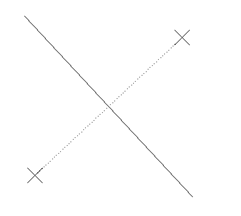
\includegraphics[scale=0.8]{tyssen1.png}	
 	\caption{Demostração da divisão em dois subespaços entre as amostras. Distância equivalente entre as duas amostras }
 	\label{tyssen1}
\end{figure}

A figura \eqref{tyssen2} demonstra a divisão de todos os subespaços entre todas as amostras mais próximas da amostra considerada. O polígono convexo é formado pela interseção de todas as linhas mais próximas da amostra em que se deseja calcular o polígono. 

\begin{figure}[H]
  	\centering
  	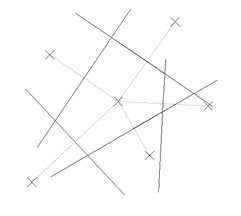
\includegraphics[scale=0.8]{tyssen2.png}	
  	\caption{Determinação do polígono convexo entre todas as amostras mais proximais da amostra considerada}
  	\label{tyssen2}
\end{figure}
 
 Cada vértice do polígono de Thyssen também pode ser determinado como o centro do círculo determinado pela amostra e dois pontos mais próximos. A figura \eqref{tyssen3} demonstra esta relação geométrica. 
 
 \begin{figure}[H]
 	\centering
 	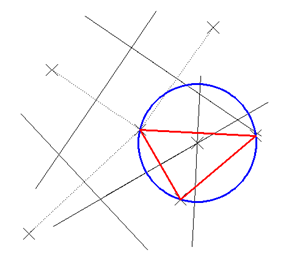
\includegraphics[scale=0.8]{tyssen3.png}	
 	\caption{Determinação do vértice do polígono de Thyssen pelo círculo determinado pela amostra considerada e duas amostras mais proximais}
 	\label{tyssen3}
 \end{figure}
 
 Cada amostra receberá então um peso igual a sua área de influência dividido pela área total de todas as amostras. A equação \eqref{pesos_area_influ} demonstra o cálculo de cada peso para cada amostra i utilizando os polígonos de influência.
 
  \begin{equation}\label{pesos_area_influ}
  \rho _{i} = \frac{A_{i}}{\sum_{i=1}^{n}A_{i}}
  \end{equation}
  
  Em que $A_{i}$ é a área ou volume de influência de cada amostra.
 
  \subsection{Método das células móveis }
  
  Outra forma de se determinar os ponderadores utilizados para o desagrupamento das amostras são as células móveis. O espaço entre as amostras é dividido em uma malha regular com n blocos. A figura \eqref{cel_m} demonstra um conjunto de amostras dividido em um grid de quatro blocos.
  
   \begin{figure}[H]
   	\centering
   	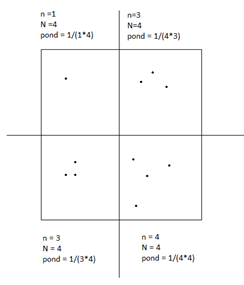
\includegraphics[scale=0.8]{celulas_moveis.png}	
   	\caption{Demonstração do método das células moveis dividindo as amostras em quatro células. Cada amostra receberá um peso como demonstrado na figura}
   	\label{cel_m}
   \end{figure}
  
  
  Cada peso de cada amostra é dado pela relação \eqref{pesos_celulasmoveis}
  
   \begin{equation}\label{pesos_celulasmoveis}
   \rho _{i} = \frac{1}{nN}
   \end{equation}
 
 Tal que n é o número de amostras contidas na célula e N é o número de células. Neste caso todas as amostras que estão contidas dentro de uma célula recebem valores iguais de peso, sendo uma desvantagem do método. O processo de desagrupamento consiste em achar o tamanho de célula que minimiza a estatística desagrupada, e para isso é necessário um processo interativo ao qual são escolhidos vários tamanhos até se determinar aquele que melhor se adequa a situação geométrica das amostras. A figura \eqref{g_cel_m} demonstra como podemos encontrar a média desagrupada a partir de um gráfico em que variamos o tamanho das células para encontrarmos o mínimo da função. O
 
 
\begin{figure}[H]
	\centering
	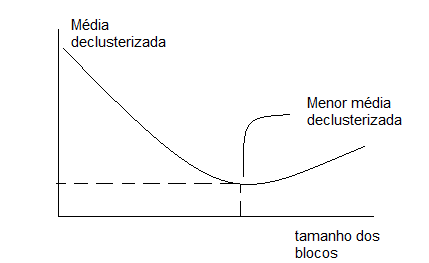
\includegraphics[scale=0.8]{grafico_celulas_m.png}	
	\caption{Demonstração do método das células moveis dividindo as amostras em quatro células. Cada amostra receberá um peso como demonstrado na figura}
	\label{g_cel_m}
\end{figure}
 
\subsection{Regularização de amostras }

Uma das condições dos métodos de estimativa e simulação utilizados na geoestatística é que as amostras devem possuir o mesmo suporte. No entanto isso nem sempre é possível na prática. Na avaliação de depósitos minerais, por exemplo, os testemunhos de sondagem apresentam tamanhos diferenciados e recuperações diferenciadas. Para isso devemos regularizar as amostras em um tamanho único e atribuir o valor médio para os testemunhos. Em casos que o suporte do volume estimado ou simulado for muito maior do que o suporte das amostras a regularização praticamente não possui efeito.

O primeiro passo para efetuar a regularização é estipular um tamanho para ser regularizado. Isso pode ser feito encontrando a moda dos valores dos tamanhos das amostras. Em seguida definimos a interseção das amostras com o suporte regularizado. A figura \eqref{regular} demonstra uma situação em que temos um minério M1 e M2. O suporte regularizado contém parte de M1 e M2.
   
\begin{figure}[H]
	\centering
	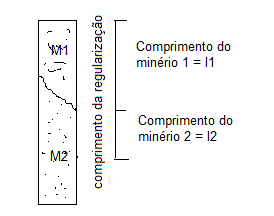
\includegraphics[scale=0.8]{regular.png}	
	\caption{Exemplo da regularização de um testemunho com dois minérios M1 e M2. Dentro do comprimento regularizado temos a partipação de um comprimento do minério 1 = l1 e um comprimento do minério 2 = l2 }
	\label{regular}
\end{figure}

Para definir, por exemplo, o teor médio do suporte regularizado, temos que realizar os cálculos segundo a equação \eqref{regularizacao_eq}

\begin{equation}\label{regularizacao_eq}
 \overline{z} = \frac{l_{1}z_{1} + l_{2}z_{2}}{l_{1}+l_{2}}
\end{equation}

Sendo $z_{1}$ e $z_{2}$ os teores médios de cada amostra e $l_{1}$ e $l_{2}$ os seus comprimentos. Na verdade apenas definimos a regularização dos teores pelo comprimento porque a seção do testemunho é a mesma para cada uma das amostras. Lidar com variáveis aleatórias regionalizadas é antes de tudo aprender a conhecer os efeitos de escala para o problema tratado. Como a dimensão do comprimento de furos de sondagem é muito maior que sua seção horizontal é considerável tratar o problema em apenas uma dimensão. 
